\documentclass[10pt,twocolumn]{article}

\usepackage[margin=0.66in]{geometry}
\usepackage{graphicx}
\usepackage{booktabs}
\usepackage{array}
\usepackage{amsmath,amssymb,amsthm}
\usepackage[switch,mathlines]{lineno}
\usepackage[hidelinks]{hyperref}
\usepackage[capitalize,noabbrev]{cleveref}

\graphicspath{{figures/}}
\setlength{\columnsep}{0.25in}
\setlength{\textfloatsep}{8pt plus 2pt minus 2pt}
\setlength{\floatsep}{6pt plus 2pt minus 2pt}
\setlength{\dbltextfloatsep}{8pt plus 2pt minus 2pt}
\setlength{\abovecaptionskip}{3pt}
\setlength{\belowcaptionskip}{0pt}
\newlength{\nmifigurewidth}
\setlength{\nmifigurewidth}{180mm}
\newlength{\nmihalffigurewidth}
\setlength{\nmihalffigurewidth}{0.485\nmifigurewidth}
\newcommand{\nmitworowpanel}[1]{\includegraphics[width=\linewidth,height=0.285\textheight,keepaspectratio]{#1}}
\newcommand{\nmithreerowpanel}[1]{\includegraphics[width=\linewidth,height=0.185\textheight,keepaspectratio]{#1}}
\renewcommand{\topfraction}{0.95}
\renewcommand{\dbltopfraction}{0.95}
\renewcommand{\textfraction}{0.05}
\renewcommand{\floatpagefraction}{0.80}
\renewcommand{\dblfloatpagefraction}{0.80}
\makeatletter
\setlength{\@fptop}{0pt}
\setlength{\@fpsep}{8pt plus 2pt}
\setlength{\@fpbot}{0pt plus 1fil}
\setlength{\@dblfptop}{0pt}
\setlength{\@dblfpsep}{8pt plus 2pt}
\setlength{\@dblfpbot}{0pt plus 1fil}
\makeatother

\newtheorem{theorem}{Theorem}
\newtheorem{proposition}[theorem]{Proposition}
\newtheorem{assumption}{Assumption}

\newcommand{\Pcal}{\mathcal P}
\newcommand{\Ncal}{\mathcal N}
\newcommand{\Fcal}{\mathcal F}
\newcommand{\Rcal}{\mathcal R}
\newcommand{\Hcal}{\mathcal H}
\newcommand{\E}{\mathbb E}
\newcommand{\Prob}{\mathbb P}
\newcommand{\ind}{\mathbf 1}
\newcommand{\FDP}{\mathrm{FDP}}
\newcommand{\FTR}{\mathrm{FTR}}
\newcommand{\FRF}{\mathrm{FRF}}
\newcolumntype{P}[1]{>{\raggedright\arraybackslash}p{#1}}
\setcounter{secnumdepth}{0}

\title{\vspace{-1.0em}Release cards for scientific AI candidate queues under scarce verification and reference drift}
\author{\begin{tabular}{c}
Yu Chen\textsuperscript{1,*,\textdagger} \quad
Jiahao Zhang\textsuperscript{1,\textdagger} \quad
Xinling Wen\textsuperscript{1} \quad
Shuai Liu\textsuperscript{2} \quad
Yawei Hou\textsuperscript{1}\\[0.25em]
\textsuperscript{1}Zhengzhou University of Aeronautics, Zhengzhou, Henan, China\\
\textsuperscript{2}University of Chinese Academy of Sciences, Beijing, China\\
\textsuperscript{\textdagger}These authors contributed equally: Yu Chen and Jiahao Zhang.\\
\textsuperscript{*}Correspondence: \href{mailto:chenyu@zua.edu.cn}{chenyu@zua.edu.cn}
\end{tabular}}
\date{}

\begin{document}
\modulolinenumbers[1]
\linenumbers
\pagenumbering{gobble}
\pagestyle{empty}
\makeatletter
\twocolumn[
\begin{@twocolumnfalse}
\maketitle

\begin{abstract}
\internallinenumbers
Artificial intelligence now proposes scientific candidates faster than they can be verified, yet these candidates already enter real workflows, where a predicted-stable crystal triggers density-functional calculations and a proposed cell link rewrites a lineage graph. What this pipeline lacks is a decision layer governing which AI-generated candidates may be released into downstream science. We introduce the release card, a certified and versioned record stating whether a frozen candidate queue may be released, must be refused for insufficient evidence, can be unlocked by further auditing, or has expired because the scientific reference changed. We give one construction, PARC, which issues release cards under one-sided partial verification and controls the expected false-release fraction of the released set without treating unverified candidates as negatives. Across cell tracking, materials screening, satellite mapping and ecological monitoring, PARC certifies reliable candidate sets and refuses high-volume requests that a ranked list would otherwise pass downstream with large error. When the materials stability reference is updated from 2022 to 2025, PARC detects that earlier certificates have expired and routes them to recertification. PARC turns AI-generated scientific top-\(K\) lists into auditable lifecycle decisions before they enter scientific records.
\end{abstract}
\vspace{0.8em}
\end{@twocolumnfalse}
]
\makeatother
\setcounter{linenumber}{9}

Machine-learning systems now propose scientific candidates at scale: links between cells across microscopy frames, inorganic crystals ranked for follow-up, buildings tracked through satellite time series, and animals detected in camera-trap imagery \cite{ulman2017objective,mavska2023cell,riebesell2025framework,xie2018crystal,van2021multi,beery2021iwildcam}.
These candidates enter downstream workflows.
A released crystal can trigger density-functional calculations, a released link can rewrite a lineage graph, and a released detection can enter a biodiversity record.
The number of candidates a model proposes now far exceeds the number a laboratory can verify, so most candidates enter scientific work only partially checked.
Standard task metrics score a model after labels are complete \cite{bernardin2008evaluating,luiten2021hota}.
They leave open whether a finite, partially verified queue may be released into a workflow.
Today that decision is made informally, by taking the top of a ranked list.

Two properties make this decision different from ordinary evaluation.
First, verification is one-sided.
A confirmed cell link or a publicly DFT-stable crystal can be trusted as a positive.
An unverified candidate lacks reliable negative status, and treating missing verification as a negative corrupts calibration exactly where high-score release decisions need evidence.
Second, scientific references move.
A crystal that is stable under one public energy hull can become unstable under a later one, and an audit protocol or an identity graph can be redefined.
A static top-\(K\) list has nowhere to record one-sided evidence, additional auditing, expiry, or recertification.

The breadth of this problem comes from a shared workflow structure across scientific AI pipelines.
Many pipelines now produce ranked finite objects that are cheaper to generate than to verify: cell-link proposals in microscopy, crystal candidates in materials screening, building correspondences in Earth observation and localized detections in ecological monitoring.
In each case, a naive top-\(K\) release can pollute a downstream scientific artifact, while exhaustive negative labeling remains unavailable.
The common missing layer is a release-card system: a versioned computational record that states whether a frozen candidate queue is certified for release, must be refused, can be unlocked by targeted one-sided audit, or has expired after a reference update.
\Cref{fig:overview} shows this lifecycle, and \Cref{tab:capability} contrasts the lifecycle states with static candidate-selection outputs.

We give one construction of this release-card layer, partial-annotation robust certification (PARC), for sparse one-sided verification.
PARC addresses the release-card problem with upstream predictors treated as inputs.
It freezes the candidate universe, removes verified positives from calibration, leaves all unverified candidates in a conservative null superset, uses block-maximum e-values to quantify release evidence and applies a denominator-aware self-consistency rule to decide whether the queue is released or refused.
PARC reuses machinery from conformal risk control and e-value selection \cite{vovk2005algorithmic,bates2021distribution,wang2022false,ramdas2023game}; its contribution is the finite lifecycle object for release, refusal, active audit, expiry, recertification and risk triage.
The contribution is a release layer for scientific AI workflows, with candidate generation, prediction, tracking, detection and ranking treated as upstream inputs.
PARC-A turns the same certificate into an audit-design tool by showing that a small targeted positive-verification budget can unlock release where random verification remains too diffuse.
Reference-drift experiments in materials screening test the other side of the lifecycle: old certificates expire before automatic inheritance under a new reference and must then refuse, recertify or enter risk triage.

The method matters because uncertified top-\(K\) release changes scientific records as well as benchmark scores.
Three results show what the release card buys.
In cell tracking, a verified-positive budget covering only 0.2\% of the calibration candidates flips a refusal into a strict certified release, whereas the same budget spent at random unlocks nothing; the framework therefore quantifies how much targeted auditing a release requires.
When a request exceeds the available evidence, PARC prevents downstream harm through certified refusal: at a high-volume materials request, a raw ranked list would pass roughly 41\% false candidates to follow-up, and PARC returns an empty certified release.
When the materials stability reference is updated from a 2022 to a 2025 energy hull, earlier certificates expire: the released sets stay less error-prone than the raw list under the new reference, but no longer meet the original target, so PARC reports expiry and recertification instead of carrying the certificate forward.

Our contributions are threefold.
(i) We introduce the release card, a certified and versioned decision object that turns an AI-generated candidate queue into a release, refusal, audit, expiry, or recertification state (\Cref{fig:overview}).
(ii) We give PARC, a construction that issues release cards under one-sided partial verification with an expected false-release-fraction guarantee, requiring no trusted negatives and no candidate-level independence (Methods; Theorems 1--2).
(iii) We show, across four scientific domains, that the same release layer certifies reliable candidate sets, refuses unsupported requests, and detects certificate expiry under reference drift.

\section{Results}

The Results are organized around the release-card lifecycle.
\Cref{fig:overview} defines the release-card object and the PARC calculus.
\Cref{tab:capability} shows the capability distinction between a release card and static top-\(K\), threshold or e-value selection outputs.
\Cref{fig:atlas} gives the primary constructive case: PARC-A targeted one-sided audit unlocks strict CTC release while matched-budget random reveal stays empty.
\Cref{fig:nohumanconsequence} supplies operating-context evidence by translating release and refusal into downstream scientific artifacts.
\Cref{fig:materials} gives the reference-drift stress test: PARC supplies certified stopping under the \(t_0\) public labels, and the later reference hull expires the old certificate while exposing durability-risk triage.
\Cref{fig:audit_envelopes} shows audited operating envelopes where the same release card supports lower-risk release and refuses unsupported requests.
\Cref{fig:governance} closes the loop with refusal attribution, assumption diagnostics and the capability ledger that distinguishes release cards from static top-\(K\) selectors.

\subsection{Release cards replace static top-\(K\) candidate lists}

PARC wraps a frozen proposal source and makes a release decision over candidate units.
The candidate unit may be a cell link, a same-building link, a detection, a path or a track; the statistical object is the released set.
\Cref{fig:overview} summarizes the mechanism.
Verified positives are removed from the unsupported pool only when the verification rule is one-sided reliable.
All remaining candidates form a null superset, which preserves validity and can limit power when many true candidates remain unverified.
PARC uses no trusted negative labels; it asks only which candidates can be safely removed as verified positives, and leaves everything else in the null superset.
Block-level calibration absorbs spatial, temporal, camera-location or video-level dependence.
The final set is released only if all retained candidates satisfy the self-consistency threshold for the requested false-release fraction.
If no non-empty compatible set satisfies the condition, PARC returns certified refusal.
The framework view also clarifies how to read the empirical tables.
A non-empty release is evidence that the chosen candidate unit, verification rule, block definition and score together support the requested release decision.
A refusal records insufficient evidence for release at the requested operating point.
Both outputs are conditional on the frozen candidate universe and protocol.
The certificate controls the expected false-release fraction of the released set under the stated assumptions; tail-probability and individual-candidate claims require additional arguments.
We use FTR for the realized false-release fraction of a finite released set; the controlled expectation is the direct analogue of FDR/FDP terminology for this release object.
\textbf{Practical checklist for claiming a conditional PARC certificate.}
PARC controls the expected false-release fraction of the released set under a frozen, covered candidate universe with one-sided reliable positives and block exchangeability.
Individual truth, recall and high-probability error are outside this set-level guarantee.
To make such a claim, define the frozen universe; predeclare \(K\), \(\alpha\), score, compatibility and blocks; verify one-sided positives; and report coverage, block sensitivity, evidence mass and refusal.
In a toy release, PARC removes only audited positives from calibration blocks, takes the maximum score among the remaining unsupported candidates in each block, converts the resulting rank p-value for a proposed test candidate into an e-value and releases a set only when every retained candidate clears \(E_p\ge K/(\alpha|R|)\).
If the unsupported block maxima are too large, the output is certified refusal.

\begin{figure*}[t]
  \centering
  \begin{minipage}[t]{0.36\linewidth}
    \textbf{a}\par\vspace{0.25em}
    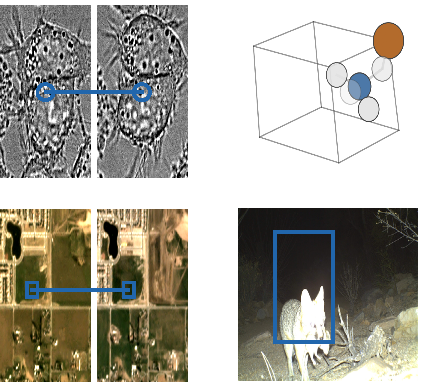
\includegraphics[width=\linewidth]{figure1_assets/rebuild/figure_1a_units_plate.pdf}
    \vspace{0.25em}
    {\scriptsize
    \setlength{\tabcolsep}{1.5pt}
    \begin{tabular}{@{}P{0.48\linewidth}P{0.48\linewidth}@{}}
      CTC cell link & WBM crystal candidate \\
      SpaceNet building link & iWildCam animal box \\
    \end{tabular}}
  \end{minipage}\hfill
  \begin{minipage}[t]{0.61\linewidth}
    \textbf{b}\par\vspace{0.25em}
    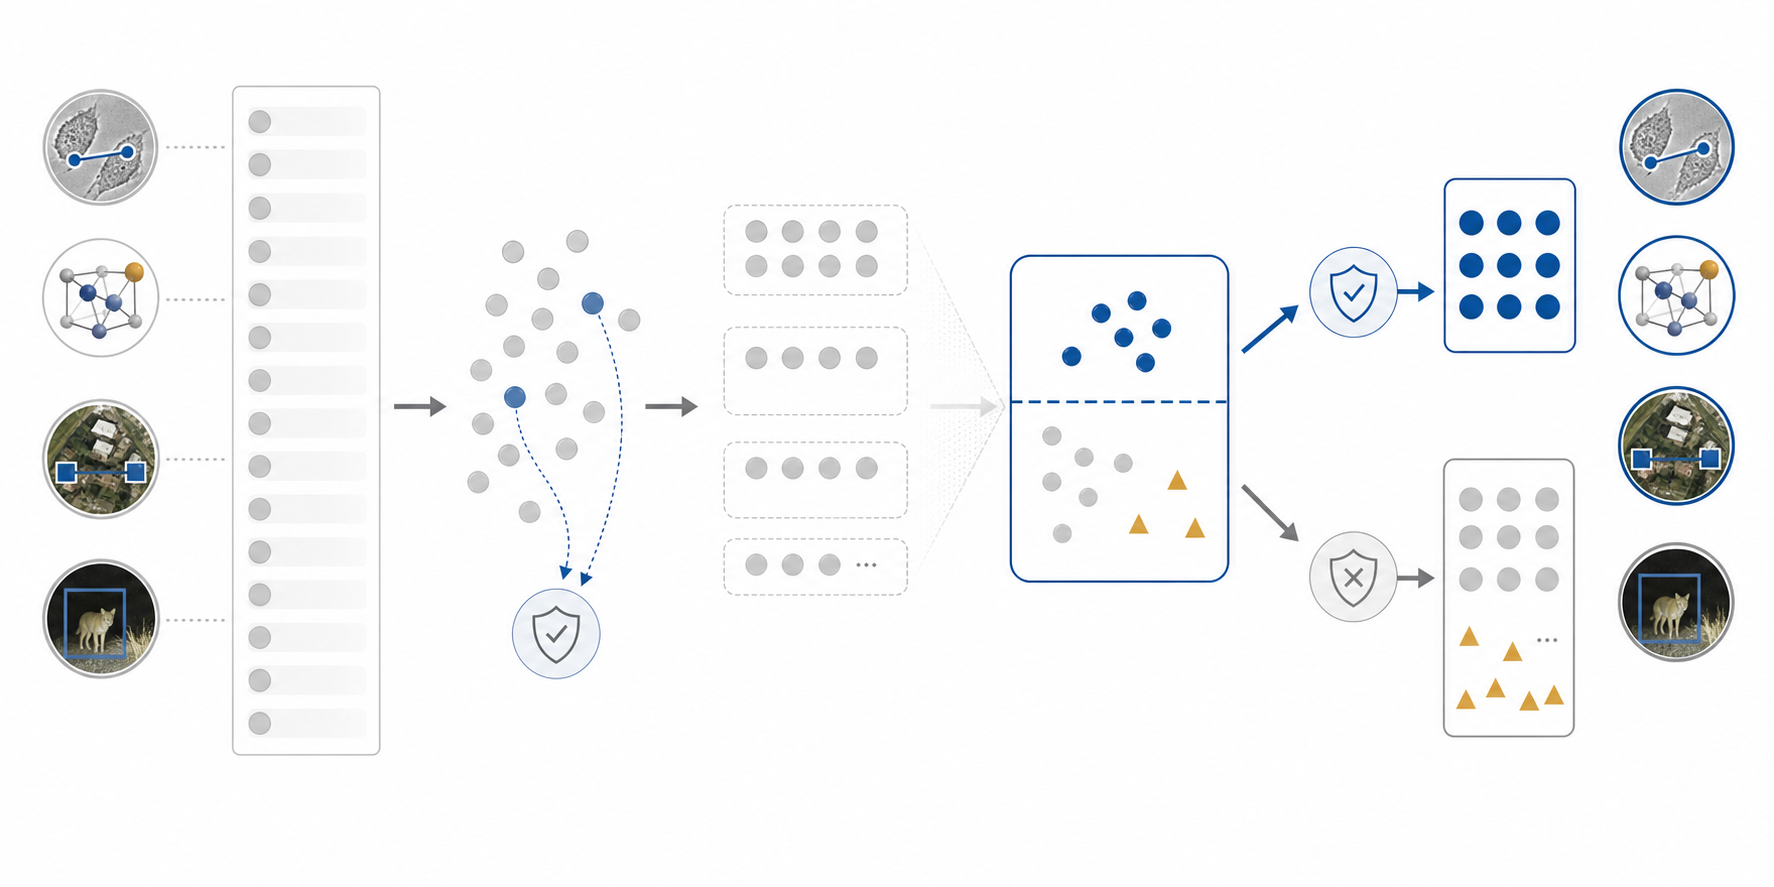
\includegraphics[width=\linewidth]{figure1_assets/rebuild/figure_1b_method_ai_backdrop.png}
    \vspace{0.25em}
    {\scriptsize
    \setlength{\tabcolsep}{1.4pt}
    \begin{tabular}{@{}P{0.18\linewidth}P{0.20\linewidth}P{0.20\linewidth}P{0.22\linewidth}P{0.15\linewidth}@{}}
      Frozen universe & One-sided support & Null-superset blocks & Self-consistency gate & Output \\
      candidate units & remove verified positives & block-max e-values & \(E_i \ge K/(\alpha |R|)\) & release or refuse \\
    \end{tabular}}
  \end{minipage}

  \vspace{2pt}
  \begin{minipage}[t]{0.47\linewidth}
    \textbf{c}\par\vspace{0.25em}
    {\scriptsize
    \setlength{\tabcolsep}{2pt}
    \renewcommand{\arraystretch}{1.10}
    \begin{tabular}{@{}P{0.22\linewidth}cP{0.22\linewidth}cP{0.22\linewidth}cP{0.22\linewidth}@{}}
      frozen queue & \(\rightarrow\) & certified release & \(\rightarrow\) & reference update & \(\rightarrow\) & expired card \\
      one-sided support &  & released set &  & new labels/hull &  & recertify/refuse \\
    \end{tabular}

    \vspace{2pt}
    \begin{tabular}{@{}P{0.31\linewidth}P{0.31\linewidth}P{0.31\linewidth}@{}}
      \(\downarrow\) active audit & \(\downarrow\) recertification & \(\downarrow\) risk triage \\
      add verified positives & rerun PARC at new reference & route fragile cards \\
    \end{tabular}}
  \end{minipage}\hfill
  \begin{minipage}[t]{0.50\linewidth}
    \textbf{d}\par\vspace{0.25em}
    {\scriptsize
    \setlength{\tabcolsep}{2pt}
    \renewcommand{\arraystretch}{1.05}
    \begin{tabular}{@{}P{0.25\linewidth}P{0.34\linewidth}P{0.34\linewidth}@{}}
      \toprule
      State & Trigger & Claim allowed \\
      \midrule
      certified release & self-consistency passes & expected FTR control \\
      certified refusal & evidence mass insufficient & no supported release \\
      active audit & limiting positives hidden & reveal one-sided support \\
      expired & reference update & old card not inherited \\
      recertified refusal & new reference fails gate & versioned safety state \\
      risk triage & drift-risk signal & route fragile cards \\
      \bottomrule
    \end{tabular}}
  \end{minipage}
  \caption{\textbf{PARC release-card lifecycle.} a, The released units are finite scientific candidates: examples show a CTC cell link, a WBM crystal candidate from the public Materials Cloud archive, a SpaceNet same-building link and an animal-present camera-trap box. b, PARC freezes the candidate universe, removes only one-sided verified positives, calibrates a conservative null superset with block maxima and applies the self-consistency threshold \(e_i\ge K/(\alpha |R|)\). c, A release card records lifecycle transitions: active audit can add one-sided support, reference updates expire old cards and recertification can release, refuse or route to risk triage. d, The miniature state ledger gives the allowed claim for each state; full truth is reserved for post-release FTR evaluation.}
  \label{fig:overview}
\end{figure*}

\begin{table*}[t]
  \centering
  \scriptsize
  \setlength{\tabcolsep}{2pt}
  \renewcommand{\arraystretch}{1.08}
  \begin{tabular}{@{}P{0.13\linewidth}P{0.17\linewidth}P{0.12\linewidth}P{0.12\linewidth}P{0.10\linewidth}P{0.10\linewidth}P{0.12\linewidth}@{}}
    \toprule
    Output layer & Native object & One-sided positives & Release/refusal & Active audit & Reference expiry & Recertification or triage \\
    \midrule
    Top-\(K\) ranked list & fixed-size prefix & absent & release only & absent & absent & absent \\
    Threshold or split conformal score rule & score or p-value threshold & limited by available labels & threshold pass/fail & absent & absent & absent \\
    e-BH-style selection & e-value selected set & e-values only & selected set; lifecycle state absent & absent & absent & absent \\
    PARC release card & frozen candidate queue with versioned state & verified-positive removal from a null superset & certified release or certified refusal & targeted one-sided audit & explicit expiry under reference update & recertification and risk triage \\
    \bottomrule
  \end{tabular}
  \caption{\textbf{Release-card capabilities versus static candidate-selection outputs.} The comparison is scoped to the lifecycle state recorded by each output layer. PARC uses e-values internally and returns a versioned release card that can release, refuse, request targeted audit, expire under reference drift, recertify or route fragile queues to risk triage.}
  \label{tab:capability}
\end{table*}

\subsection{A 0.2\% targeted one-sided audit unlocks certified CTC release}

In time-lapse microscopy, released cell links become the lineage evidence used for downstream cell-motion and division analyses.
The Cell Tracking Challenge (CTC) experiment treats an adjacent-frame cell link as the unit of scientific release \cite{ulman2017objective,mavska2023cell}.
\Cref{fig:atlas} shows the positive-reveal transition, strict \(K\)-sweep, refusal controls and split/leakage diagnostics.
The strongest CTC source is a sequence-disjoint learned-hybrid linker: a scorer trained on sequence 01 is frozen before certification on held-out sequence 02.
It uses geometric features together with crop appearance and correlation signals, while GT and matching-leakage fields are excluded.
The held-out learned universe contains 146,230 candidate links, including 29,306 GT-supported links.
Full tracking truth is reserved for post-release evaluation; during calibration, PARC sees only a masked subset of true links as verified positives.
Rows with \(\rho=1.0\) are full-verification oracle diagnostics and are excluded from the abstract, primary table and main positive claims.
The release certificate attaches to the finite set of links released from this frozen candidate list.

Under \(\rho=0.10\) top-score partial verification and the strict target \(\alpha=0.10\), the learned-hybrid source releases non-empty sets in 20/20 calibration-mask seeds for \(K\in\{10,25,50,75,100,300\}\), with held-out FTR 0.000 throughout.
At \(K=100\), the release contains 100 links in every seed; the maximum observed e-value is 13.38 against a required threshold of 10, giving evidence mass 1.34.
The raw top-\(K\) slice is also clean in this small-volume regime; PARC adds the missing release statement under partial verification.
It certifies the high-confidence AI-assisted slice while observing only 10\% of true links during calibration.

The masked-label positive-reveal frontier makes this targeted-verification effect quantitative.
In these masked-label rows, the budget is a verified-positive reveal budget over the calibration-candidate universe: the frozen score orders the reveal policy, only true links selected by that policy enter PARC as observed positives, and all unrevealed or non-positive candidates remain in the null superset for calibration.
This measures how much one-sided positive support is needed for release under the frozen protocol.
The primary strong-positive row is CTC \(K=100\): score-targeted reveal reaches strict seed-stable release at a 0.2\% calibration-candidate budget, with 20/20 non-empty safe seeds, mean release size 99.15 links per seed and observed FTR 0.000.
At the same reveal budget, random reveal releases in 0/20 seeds; in the frozen grid, random reveal requires full calibration-set reveal to reach the corresponding transition.
The mechanism is visible in the calibration blocks.
At \(K=100\) and the 0.2\% budget, score-targeted positives remove 73.0 limiting positive block maxima on average, whereas random reveal removes 0.4; this 182.5-fold block-maximum removal rate explains why only the targeted row crosses the release threshold.
The CTC \(K=300\) audit-budget row is classified as support-only because it is 19/20 safe.
This establishes budget efficiency for score-targeted reveal in the frozen CTC grid.

Three checks guard against reading this as a leakage artifact.
First, the leakage audit records no train--evaluation sequence overlap, no GT identity or matching-label fields in the score, training-sequence-only normalization and a scorer frozen before PARC.
Second, the reverse split, trained on sequence 02 and certified on held-out sequence 01, gives the same \(20/20\) non-empty result with held-out FTR 0.000 across \(K=10\)--300.
Third, a random-score negative control preserves candidate identities, labels and blocks while destroying ranking evidence; its raw top-\(K\) false-link fractions are 0.76--0.81, and PARC refuses every row at \(\alpha=0.10\) and \(\alpha=0.20\).
Release requires enough calibrated evidence from the frozen score.

At high requested volume, refusal becomes the safety result.
The transparent geometric source is retained as secondary context: at \(\rho=0.10\), \(K=100\) and \(\alpha=0.20\), it releases 100 links in 20/20 calibration-mask seeds with held-out FTR 0.000, whereas random verification at the same operating point releases nothing.
For the unsafe geometric \(K=5000\) request, PARC refuses in 20/20 calibration-mask seeds, whereas the raw top-\(K\) list has actual FTR 0.3606.
The CTC experiments show strict release from an AI-assisted source, split and leakage robustness, and principled refusal when either the score or requested volume is unsuitable.

\begin{figure*}[t]
  \centering
  \begin{minipage}[t]{\nmihalffigurewidth}
    \textbf{a}\hfill{\scriptsize\textbf{0.2\% targeted transition}}\par
    {\scriptsize random: full reveal only \quad block-max removal: 182.5-fold}\par\vspace{1pt}
    \nmitworowpanel{figure2_assets/rebuild/figure_2a_active_audit_density.pdf}
  \end{minipage}\hfill
  \begin{minipage}[t]{\nmihalffigurewidth}
    \textbf{b}\par\vspace{1pt}
    \nmitworowpanel{figure2_assets/rebuild/figure_2b_strict_k_sweep_density.pdf}
  \end{minipage}

  \vspace{2pt}
  \begin{minipage}[t]{\nmihalffigurewidth}
    \textbf{c}\par\vspace{1pt}
    \nmitworowpanel{figure2_assets/rebuild/figure_2c_refusal_controls_density.pdf}
  \end{minipage}\hfill
  \begin{minipage}[t]{\nmihalffigurewidth}
    \textbf{d}\par\vspace{1pt}
    \nmitworowpanel{figure2_assets/rebuild/figure_2d_reverse_leakage_density.pdf}
  \end{minipage}
  \caption{\textbf{A 0.2\% score-targeted one-sided reveal unlocks CTC release, whereas random reveal requires full verification.} a, The positive-reveal operating surface is shown as seed-level mini plots across audit budget, source policy, risk level, \(K\), release fraction, held-out FTR and evidence mass; the visual anchors mark the targeted transition, the random full-reveal transition and the 182.5-fold block-maximum removal mechanism. b, The strict learned-source surface shows release, FTR, raw FTR, evidence mass and e-value margin across requested \(K\) and verification fraction. c, Official-ground-truth lineage consequences are shown as source-resolved \(K\)-sweeps of false-edge, component, edit-burden, false-fraction and release metrics. d, Primary, reverse-split and destroyed-ranking controls are shown as matched metric grids, with held-out scorer diagnostics below.}
  \label{fig:atlas}
\end{figure*}

\subsection{Operating-context consequences of release and refusal}

The operating-context question is whether the release interface changes the scientific object passed downstream.
We therefore evaluate consequence-level endpoints using only public labels, official ground truth or existing model predictions, without introducing new human audit.
In materials screening, the endpoint is the composition of a computational follow-up queue; in CTC, it is false lineage-edge insertion and component corruption; and in SpaceNet 7, it is false same-building persistence links.
These analyses translate the same certified release/refusal decisions into the artifacts that downstream scientists would actually use.
\Cref{fig:nohumanconsequence} summarizes these consequence-level endpoints as quantitative grids.

\begin{figure*}[t]
  \centering
  \begin{minipage}[t]{\nmihalffigurewidth}
    \textbf{a}\par\vspace{1pt}
    \nmitworowpanel{figure6_assets/rebuild/figure_6a_materials_artifact_grid.pdf}
  \end{minipage}\hfill
  \begin{minipage}[t]{\nmihalffigurewidth}
    \textbf{b}\par\vspace{1pt}
    \nmitworowpanel{figure6_assets/rebuild/figure_6b_ctc_artifact_grid.pdf}
  \end{minipage}

  \vspace{2pt}
  \begin{minipage}[t]{\nmihalffigurewidth}
    \textbf{c}\par\vspace{1pt}
    \nmitworowpanel{figure6_assets/rebuild/figure_6c_map_audit_grid.pdf}
  \end{minipage}\hfill
  \begin{minipage}[t]{\nmihalffigurewidth}
    \textbf{d}\par\vspace{1pt}
    \nmitworowpanel{figure6_assets/rebuild/figure_6d_release_card_quant_grid.pdf}
  \end{minipage}
  \caption{\textbf{Release certificates change computational science artifacts without new human labels.} a, Retrospective public-label materials follow-up emulation combines seed-level raw/PARC/prevented queue distributions with public-label model/budget frontiers. b, CTC official-ground-truth lineage consequences are shown as source-resolved \(K\)-sweeps of false-edge, component, release and evidence-mass metrics. c, SpaceNet 7 building-persistence consequences are shown as source-resolved \(K\)-sweeps of false-link, map-edit and release metrics. d, Release-card summaries are encoded as quantitative metric grids.}
  \label{fig:nohumanconsequence}
\end{figure*}

In the fixed-budget materials follow-up analysis, ALIGNN-FF raw top-500 would send 163.4 unstable candidates to computational follow-up per calibration-mask seed; PARC releases 90.8 candidates with 5.2 unstable candidates, preventing 158.3 unstable follow-ups relative to the requested raw queue.
The matched-size raw prefix has the same FTR as the certified queue, so the operational value is certified stopping from one-sided calibration evidence and refusal for unsupported queue sizes.
At \(K=5000\), the raw list would send 2,577.4 unstable candidates to follow-up per seed, while PARC returns certified refusal.
Across the local public materials model-zoo frontier, CGCNN, ALIGNN-FF and MEGNet show different raw-risk and power profiles; the same release interface applies, with supported budgets producing certified queues and unsupported high-volume requests returning refusal \cite{chen2019graph}.
At \(\alpha=0.10,K=500\), the CGCNN, ALIGNN-FF and MEGNet certified queues prevent 158.25, 158.3 and 105.4 unstable follow-ups per seed, respectively; at \(K=5000\), refusal prevents 2,032.6, 2,577.4 and 2,683.5 unstable follow-ups per seed.
The release-frontier model-zoo table reports only sources with local public prediction files under the same provenance constraints; the CHGNet/MACE single-point score audit below is a separate support-proxy analysis.

The same consequence view applies outside materials.
For CTC, the noisy high-volume raw \(K=5000\) queue inserts 2,907.5 false lineage edges per seed, and the random-score \(K=5000\) queue inserts 3,997.1 false lineage edges per seed; PARC refusal prevents these false edges from entering the released lineage graph.
For SpaceNet 7, the identity-preserving randomized same-building stress source inserts 3,398.9 false persistence links per seed at \(K=5000\), quantifying avoidable building-persistence map pollution under refusal.
Thus the main consequence of PARC is a changed scientific decision: which candidates are allowed to enter a downstream workflow under partial verification.

\subsection{Reference-neighborhood state predicts materials certificate fragility}

Retrospective materials screening provides the clearest reference-drift stress test for release-card lifecycle decisions.
A learned model ranks inorganic crystal candidates for possible follow-up, but every released candidate can trigger DFT calculation, literature triage or experimental planning.
We instantiate PARC on the public Matbench Discovery/WBM setting, where the release unit is one WBM unique prototype and the validity event is DFT stability at \(e_{\mathrm{above\ hull}}\le 0\) eV per atom \cite{riebesell2025framework}.
The frozen candidate universe contains 215,486 prototypes, of which 32,942 are DFT-stable under the public labels.
The primary source is a public CGCNN 10-member ensemble materials model \cite{xie2018crystal}.
Its score is negative predicted energy above hull, computed from public predicted formation energies and the WBM hull reference.
DFT stability labels are not used for ranking; they are masked to create observed positives for PARC and then used after release to compute held-out actual FTR.
The primary block is a chemistry-aware composition-family pair, with exact chemical-system and Wyckoff-family blocks retained as sensitivity checks.
\Cref{fig:materials} combines the materials release frontier, matched-volume baseline comparison, seed variability and robustness diagnostics.

\begin{figure*}[t]
  \centering
  \begin{minipage}[t]{\nmihalffigurewidth}
    \textbf{a}\par\vspace{1pt}
    \nmithreerowpanel{figure3_assets/rebuild/figure_3a_model_budget_ftr_grid.pdf}
  \end{minipage}\hfill
  \begin{minipage}[t]{\nmihalffigurewidth}
    \textbf{b}\par\vspace{1pt}
    \nmithreerowpanel{figure3_assets/rebuild/figure_3b_followup_count_grid.pdf}
  \end{minipage}

  \vspace{2pt}
  \begin{minipage}[t]{\nmihalffigurewidth}
    \textbf{c}\par\vspace{1pt}
    \nmithreerowpanel{figure3_assets/rebuild/figure_3c_seed_distribution_grid.pdf}
  \end{minipage}\hfill
  \begin{minipage}[t]{\nmihalffigurewidth}
    \textbf{d}\par\vspace{1pt}
    \nmithreerowpanel{figure3_assets/rebuild/figure_3d_baseline_alternative_grid.pdf}
  \end{minipage}

  \vspace{2pt}
  \begin{minipage}[t]{\nmihalffigurewidth}
    \textbf{e}\par\vspace{1pt}
    \nmithreerowpanel{figure3_assets/rebuild/figure_3e_threshold_robustness_grid.pdf}
  \end{minipage}\hfill
  \begin{minipage}[t]{\nmihalffigurewidth}
    \textbf{f}\par\vspace{1pt}
    \nmithreerowpanel{figure3_assets/rebuild/figure_3f_gamma_block_control_grid.pdf}
  \end{minipage}
  \caption{\textbf{Materials release cards stop raw-unsafe \(t_0\) queues but expire under current-MP reference drift.} a, Model-by-budget FTR mini charts compare raw top-\(K\), matched-size raw top-\(R\) and PARC across the available public model sources. b, The corresponding follow-up-count mini charts show raw unstable, PARC unstable and prevented unstable candidates. c, Seed-level FTR distributions expose variability behind the mean release-policy frontier. d, Nearest practical alternatives compare FTR and release size for the baseline rows used in the main text. e, Stability-definition robustness traces FTR, release fraction and evidence mass across supported and boundary rows. f, Gamma, block and refusal-control diagnostics show calibration sensitivity without turning protocol-only, current-MP drift or random-score rows into headline positive evidence.}
  \label{fig:materials}
\end{figure*}

Public ALIGNN-FF WBM predictions give the strongest practical contrast.
At \(K=300\), the raw top-\(K\) list has FTR 0.253, corresponding to about 76 unstable candidates in a 300-candidate follow-up queue; PARC releases a mean of 115 candidates with FTR 0.087, about 10 unstable candidates in the certified release set.
At \(K=500\), the raw top-\(K\) list has FTR 0.327, about 163 unstable candidates, while PARC releases a mean of 91 candidates with FTR 0.048, about four unstable candidates.
Matched-volume diagnostics give the same FTRs for the raw prefix truncated to the PARC release size.
The claim is operational: PARC uses partial verification to stop the requested queue at a certified size and to refuse unsupported volume.
Equivalently, the full raw \(K=500\) queue has follow-up cost per stable candidate \(1/(1-\mathrm{FTR})=1.49\), whereas both the certified queue and the matched-size raw prefix have cost about 1.06; this cost diagnostic records the value of stopping relative to the requested raw queue.

A clean empirical-baseline frontier sharpens this comparison against practical alternatives.
Across 11 baseline families, including raw top-\(K\), raw top-\(R\), thresholding, split conformal, post-filter e-values, e-BH-style selection, nnPU, Bao-style selective conformal and oracle diagnostics, the materials result remains a certified stopping claim.
For ALIGNN-FF \(K=300\), raw top-\(K\) FTR is 0.253, PARC and matched-size raw top-\(R\) both have FTR 0.087, and certified stopping avoids 64.25 unstable follow-ups relative to the requested queue.
For ALIGNN-FF \(K=500\), raw top-\(K\) FTR is 0.327, PARC and raw top-\(R\) both have FTR 0.048, and the avoided unstable follow-up count is 158.30.
For CGCNN \(K=500\), raw top-\(K\) FTR is 0.326 and a post-filter e-value rule reduces it to 0.163, whereas PARC and raw top-\(R\) reach 0.032 under the same retrospective public-label evaluation.

We next asked whether the materials release decisions retained utility after the reference hull changed.
This out-of-time audit evaluates utility under a later truth definition while keeping formal certification tied to the original reference.
We froze the WBM/Matbench queue candidates and PARC decisions calibrated against the local \(t_0\) snapshot, defined by MP v2022.10.28 hull labels, and re-evaluated the same released and raw queue candidates against the current Materials Project API snapshot dated 2025.09.25.
The audit covers 1,191 frozen \(K=300/500\) WBM queue candidates, 774 chemical systems and 29,279 Materials Project entries.
Under the current-MP hull, PARC retained a lower false-release burden than the requested raw top-\(K\) queues.
At \(K=300\), current-MP FTR was 0.316 for PARC versus 0.422 for raw top-\(K\), a reduction of 0.106.
At \(K=500\), current-MP FTR was 0.310 for PARC versus 0.487 for raw top-\(K\), a reduction of 0.177.
Stable-to-unstable drift also remains lower in the PARC releases: drift rates were 0.184 versus 0.213 at \(K=300\) and 0.204 versus 0.222 at \(K=500\) for PARC and raw top-\(K\), respectively.
Current-MP FTR remains above the original \(\alpha=0.10\) target, so the old card expires under the later reference.
The result shows practical queue-level utility under a public reference-hull update, while certification remains tied to the truth definition used for calibration.

The version shift also reveals a reliability finding hidden from the \(t_0\) certificate alone.
Stable-to-current-unstable drift is weakly predicted by the released candidate's own \(t_0\) margin or rank: candidate margin gives AUC 0.544 and raw rank gives AUC 0.467 in the durability-risk diagnostic.
In contrast, \(t_0\) chemical-system state predicts which certificates are fragile under the later hull, with system-level features reaching AUC 0.766.
The strongest interpretable signal is the chemical-system margin distribution, with AUC 0.844; raw near-hull density alone is near random at AUC 0.502 and is treated as an Extended Data negative ablation.
The pruned headline model, using \(t_0\)-only margin-distribution plus size/activity features and grouped cross-validation by chemical system, gives AUC 0.809 with a chemical-system bootstrap 95\% CI of 0.722--0.874.
It flags 67\% of observed stable-to-current-unstable flips in the top 30\% high-risk group, while a train-fold base-rate control has AUC 0.500.
This is a release-card risk-triage signal for recertification.
It uses only \(t_0\)-available features at deployment time and leaves independent DFT validation outside the claim.
The strongest PARC-D retained subset is therefore reported as risk triage.
The locked row retains 89 candidates with observed current-MP FTR 0.022 and a 95\% \(\alpha_0+\beta_{\mathrm{UCB}}\) bound below 0.10, yet the retained post-filter set fails PARC self-consistency because its minimum e-value remains below the threshold induced by the smaller retained denominator.
PARC-D routes high-risk rows to recertification without inheriting PARC alpha-control after post-filtering.

Candidate-level explanation shows where the remaining current-label failures occur.
At \(K=300\), the 96 conservative current-MP false candidates in the PARC release comprise 72 ALIGNN-FF disagreements with the later hull label, 15 near-hull boundary cases under 25--50 meV per atom windows and 9 unresolved current-MP reference cases counted conservatively as false.
At \(K=500\), the corresponding 67 PARC false candidates comprise 56 ALIGNN-FF disagreements, 7 near-hull boundary cases and 4 unresolved current-MP reference cases.
No PARC current-MP false candidate in this diagnostic is both far from hull and ALIGNN-negative under the available public prediction source.
CHGNet and MACE-MP candidate-level scores are now available for the frozen WBM queue as an auxiliary score-support audit.
At \(K=300\), the CHGNet/MACE consensus-support proxy is 0.812 for the PARC release and 0.590 for the raw-only extra-tail; at \(K=500\), the corresponding values are 0.847 and 0.632.
These raw-energy-per-atom proxies support the interpretation that the released subset is stronger than the raw-only extra-tail under auxiliary models.
Their scope is score support: they are outside reference-hull \(e_{\mathrm{above\ hull}}\), DFT validation, prospective discovery and strict current-MP certification.
A simple CHGNet/MACE support gate also leaves the \(t_1\) FTR materially unrepaired, so this audit remains score-support evidence.

The corresponding materials audit-budget frontier defines a boundary case.
For ALIGNN-FF \(K=300/500\), top-score reveal at 0.5\% reaches a mean-operating transition, but seed-level \(\alpha\)-violation rates of 0.45 and 0.15 keep these rows out of the strict headline.
They show that materials follow-up requires stronger verification or source-aware audit before the audit-budget result can be read as a seed-stable release claim.

At \(\rho=0.10,\alpha=0.10,K=100\), the predeclared CGCNN endpoint releases in 20/20 calibration-mask seeds with mean release size 100 and held-out actual FTR 0.030.
The raw top-\(K\) slice at this small budget is already stable under the public labels, so this row serves as a calibration and validity check: PARC remains below the \(\alpha=0.10\) budget and attaches a set-level certificate.
The practical value claim comes from raw-unsafe larger budgets and refusal rows.
The larger CGCNN \(K=300\) row also releases in 20/20 calibration-mask seeds with mean actual FTR 0.0916 and is treated as sensitivity because it is closer to the risk budget and has greater seed-level variability.
At \(K=5000\), PARC refuses in 20/20 calibration-mask seeds while the raw top-\(K\) list has actual FTR 0.4065, showing that a strong learned materials ranking still needs bounded release.

We also report matched-volume diagnostics for the ALIGNN headline rows and CGCNN near-boundary rows.
When raw is truncated to the same average release size as PARC, raw top-\(R\) and PARC have the same realized FTR for these prefix-like releases; the reduction relative to raw top-\(K\) comes from issuing a smaller certified queue.
Post-filter e-threshold and split-conformal comparator rows at the same requested budgets remain empirical filters without the PARC set-level release/refusal certificate.

Controls guard the interpretation.
The leakage audit records that public precomputed predictions are used, DFT target labels are not used for ranking, and full DFT labels enter only observed-positive masking and held-out FTR evaluation.
Random-score controls on the same candidate universe refuse at \(\alpha=0.10\) for \(K=300\) and \(K=1000\), where raw top-\(K\) actual FTR is about 0.85.
Public ALIGNN-FF WBM predictions also show that the release-wrapper behavior is not specific to CGCNN.
The materials result is stable across the main stability definitions and calibrator diagnostics.
Across exact-stable, 25 meV tolerance-positive, 25 meV margin-excluded and conservative clear-stable definitions, the main low-volume conclusions remain stable, while boundary rows expose where the scientific definition of stability begins to matter.
In particular, the ALIGNN margin-excluded 25 meV setting at \(K=100\) is reported as a boundary sensitivity with realized FTR near the risk budget.
Fixed-\(\gamma\) grids are reported as power diagnostics: any fixed \(0<\gamma<1\) is a valid e-calibrator, and the finite-resolution rule for choosing \(\gamma\) uses calibration resolution.
Weak-model, block-sensitivity, threshold-sensitivity, fixed-\(\gamma\) and high-volume refusal rows are reported in Extended Data and the Supplement.
The claim is a retrospective candidate-release certificate for public WBM stability labels: it governs which frozen model candidates are statistically licensed for release or follow-up under partial DFT verification.

\subsection{Audited operating envelopes expose release-card boundaries}

\begin{figure*}[t]
  \centering
  \begin{minipage}[t]{\nmihalffigurewidth}
    \textbf{a}\par\vspace{0.15em}
    \nmitworowpanel{figure4_assets/rebuild/figure_4a_iwild_audit_microplots.pdf}
  \end{minipage}\hfill
  \begin{minipage}[t]{\nmihalffigurewidth}
    \textbf{b}\par\vspace{0.15em}
    \nmitworowpanel{figure4_assets/rebuild/figure_4b_iwild_operating_surface.pdf}
  \end{minipage}

  \vspace{2pt}
  \begin{minipage}[t]{\nmihalffigurewidth}
    \textbf{c}\par\vspace{0.15em}
    \nmitworowpanel{figure4_assets/rebuild/figure_4c_spacenet_audit_surface.pdf}
  \end{minipage}\hfill
  \begin{minipage}[t]{\nmihalffigurewidth}
    \textbf{d}\par\vspace{0.15em}
    \nmitworowpanel{figure4_assets/rebuild/figure_4d_spacenet_map_consequence_grid.pdf}
  \end{minipage}
  \caption{\textbf{Human-audit and SpaceNet operating envelopes.} a,b, The iWildCam internal-audit row is shown as block-level audit distributions and operating-surface metrics over \(K\), risk level and random-score controls. c,d, SpaceNet real-audit and official map-consequence diagnostics show release fraction, evidence mass, official FTR, audit coverage and downstream false-persistence-link consequences.}
  \label{fig:audit_envelopes}
\end{figure*}

Camera-trap monitoring tests whether localized animal detections can satisfy the assumptions needed for ecological candidate release under strong location shift \cite{beery2021iwildcam,koh2021wilds}.
The downstream scientific object is a candidate animal observation, and the operational question is whether a small audited queue can support release of animal-present detections.
\Cref{fig:audit_envelopes} places this ecological audit beside the SpaceNet audit/refusal envelope.

The species-level setting fails the one-sided reliability condition needed for localized release.
Open-vocabulary species prompts can localize the wrong animal, part of an animal or background while being weakly supported by image-level species metadata.
Such support violates the verified-positive implication \(A_p=1\Rightarrow Y_p=1\) for localized detections.
Under this semantic mismatch, the release card rejects the verification rule.

Human verification changes the animal-present result from a proxy-label power limit into an operational ecological release.
The frozen iWildCam animal-present source produced 17,169 candidates across 6,000 images and 30 camera locations.
In the calibration audit, 1,414 of 2,000 candidates were human-confirmed animal detections and 586 were not animal, with no uncertain labels; only the animal labels entered PARC as one-sided verified positives.
This audit composition reflects the pre-specified audit queue.
Using those human-confirmed positives, PARC released at the operational point \(\alpha=0.20,K=50\) in 20/20 fixed-protocol audit seeds, with mean release size 50.
A separate internal blind release audit found 167/167 unique released candidates to be animals, giving human FTR and conservative human FTR of 0.000.
The raw top-\(K\) audit also found 300/300 animal-present candidates, which shows that the frozen detector supplies a clean high-score animal-present slice; PARC attaches an auditable release certificate to that slice using only the human-confirmed positives available to the calibration protocol.

The strict-risk boundary remains important.
At \(\alpha=0.10\), the internally audited animal-present rows for \(K=25,50\) and 100 all return certified refusal because the maximum observed e-value, 6.456, remains below the required threshold 10.
iWildCam therefore contributes an internally audited operating point: an ecological animal-present release at \(\alpha=0.20,K=50\), paired with species-level reliability and strict-risk refusals that define the operating envelope.
Together, these rows define the ecological operating envelope: valid release requires both reliable one-sided positives and enough evidence at the requested operating point; when either condition is missing, refusal is the scientific output.



\subsection{SpaceNet separates low-volume release from high-volume refusal}

In satellite-based urban monitoring, same-building links determine whether a footprint persists, appears or disappears across time.
SpaceNet 7 instantiates PARC on this Earth-observation release unit \cite{van2021multi}.
We construct adjacent-time same-building links from 18 areas of interest, yielding 6,341,788 candidate links and 2,050,769 GT-supported links.
The geometry linker is a structured proposal source, whereas a randomized linker provides an unsafe-source stress test.
As in CTC, partial-verification rows hide most true links from PARC and evaluate held-out actual FTR only after release.
The scientific unit here is a same-building correspondence that may feed persistence, demolition or construction summaries.
This makes SpaceNet a useful contrast to CTC: the candidate universe is much larger, the blocks are organized by AOI and time, and the proposal source can be either a meaningful geometric heuristic or a deliberately corrupted linker.
The certification problem, however, is identical at the release layer.

At \(\rho=0.10\), \(\alpha=0.20\) and \(K=100\), the geometry linker releases a mean of about 82 links in 17/20 calibration-mask seeds with held-out actual FTR 0.003.
This falls one seed below the predeclared 18/20 non-empty gate and is reported as a relaxed masked-label operating check.
The raw top-\(K\) geometry list at \(K=100\) also has low held-out FTR 0.003, so this row demonstrates certification of a reliable high-confidence portion of a large Earth-observation candidate universe.
That distinction is important for interpretation: PARC attaches a release statement when the high-confidence part of the candidate universe has sufficient evidence, and refuses when the requested volume exceeds that support.
At larger budgets the geometry source eventually refuses, showing that certification is a bounded release decision.

The same protocol refuses an intentionally degraded source.
For the randomized linker, PARC releases no links, while the raw top-\(K\) false-link rates are 0.6575 at \(K=100\), 0.681 at \(K=300\) and 0.678 at \(K=500\).
SpaceNet demonstrates both sides of the release interface: low-error release from a structured proposal source and certified refusal for a mostly false raw candidate list.
The randomized stress row is a guardrail check: when upstream evidence is not separable enough, the certified output is empty even though a naive system would still return a long ranked list.

We also ran a protocolized SpaceNet human-audit loop using actual partial verification.
An 800-candidate calibration audit supplied one-sided same-building positives; unconfirmed links were not trusted negatives.
The pre-registered \(K=100,\alpha=0.20\) audit request produced certified refusal in 20/20 fixed-protocol audit seeds, showing that human verification did not license the original release volume.
A pre-specified \(K=50\) diagnostic row released in 18/20 fixed-protocol audit seeds with mean size 43.95.
Separate internal blind visual review of 147 unique released candidates found human FTR 0.000 with no uncertain cases; uncertain-as-false and official-proxy FTR were also 0.000.
Real audit supports the release/refusal workflow: PARC refuses the pre-registered \(K=100\) audit request and supports the lower-volume \(K=50\) release.
The corresponding block diagnostics, reported in the Supplement, show that the \(K=100\) audit refusal was not caused by missing AOI-time audit coverage; the limiting factor was insufficient evidence mass for the requested release volume.

\subsection{Capability and evidence-scope diagnostics close the lifecycle}

The cross-domain evidence forms a success-domain diagnostic.
Across completed rows, release and refusal are largely explained by measurable certification features: evidence mass, maximum e-value relative to the required threshold, coverage of the calibration blocks, raw top-\(K\) risk and compatibility pressure.
The descriptive success-domain map is included in the diagnostic display.
Rows with sufficient evidence mass and max-e resolution support release; rows below these gates refuse even when a naive ranked list would return candidates.
A simple descriptive rule using \(\Phi\ge 1\) and \(e_{\max}\ge e_{\mathrm{req}}\) captures the practical distinction between power-supported release and principled refusal better than domain identity alone; the theorem remains the self-consistency guarantee.
This converts the generality claim from ``PARC was tried on many datasets'' into a diagnostic statement about when the release interface has power.

The durability-risk result also has a controlled mechanism check.
We simulated evolving-reference regimes in which reference drift is either candidate-driven or neighborhood-driven, then asked which feature family predicts stable-to-current-unstable flips under group splits.
In the candidate-driven regime, candidate features dominate (AUC 0.859) and system features are near random (AUC 0.517).
In the neighborhood-driven regime, system features dominate (AUC 0.784) while candidate features are near random (AUC 0.504).
The materials pattern matches the second regime: fragility tracks the candidate's unstable reference neighborhood.
This controlled simulation is a mechanism demonstration for expiry and risk-triage states.

Candidate-level ablation reruns directly test whether verified-positive removal is load-bearing in the primary scientific rows.
Across six CTC/materials target rows and 360 seed-level reruns, leaving verified positives inside the calibration null or removing the same number of random positives reduces release in all six rows.
For CTC learned \(K=100/300\), Full PARC releases 100/300 links whereas no-removal and random-removal release none.
For ALIGNN-FF materials \(K=300/500\), Full PARC releases 115.1/90.75 candidates on average, whereas no-removal and random-removal release none; the CGCNN \(K=100\) calibration row falls from 100 to 36.75.
The ALIGNN margin-excluded 25 meV \(K=100\) row also loses release power under the ablations and remains a boundary-sensitivity row.
Thus verified-positive removal is both a formal one-sided annotation requirement and a power-critical component of the completed CTC/materials release frontiers.

Refusal has diagnostic structure.
The refusal diagnosis table separates finite-resolution caps from pre-graph evidence-mass failures and selector/compatibility limitations.
For CTC random-score and iWildCam strict \(\alpha=0.10\), the maximum observed e-value remains below the required threshold; for materials \(K=5000\) and SpaceNet human-audit \(K=100\), aggregate evidence mass is below the self-consistency requirement.
The ILP feasibility oracle is negative for these reported rows, showing that SCS-Greedy did not hide a feasible compatible release set.
If a future row were ILP-feasible while greedy remained empty, the row would be diagnosed as selector-power limitation.
The adversarial release-stress package reaches the same conclusion from the other side: score corruption, unsafe high-\(K\) requests and block-shift/downsampled stresses are completed diagnostics, and unsupported rows shrink or refuse.
The diagnostic matrix in \Cref{fig:governance} makes the same point from the other side: each row has a stated unit, one-sided positive-support mechanism, block definition, coverage policy, failure mode and claim scope.

\begin{figure*}[t]
  \centering
  \begin{minipage}[t]{\nmihalffigurewidth}
    \textbf{a}\par\vspace{1pt}
    \nmithreerowpanel{figure7_assets/rebuild/figure_7a_success_domain_metric_grid.pdf}
  \end{minipage}\hfill
  \begin{minipage}[t]{\nmihalffigurewidth}
    \textbf{b}\par\vspace{1pt}
    \nmithreerowpanel{figure7_assets/rebuild/figure_7b_verified_positive_ablation_grid.pdf}
  \end{minipage}

  \vspace{2pt}
  \begin{minipage}[t]{\nmihalffigurewidth}
    \textbf{c}\par\vspace{1pt}
    \nmithreerowpanel{figure7_assets/rebuild/figure_7c_refusal_diagnosis_grid.pdf}
  \end{minipage}\hfill
  \begin{minipage}[t]{\nmihalffigurewidth}
    \textbf{d}\par\vspace{1pt}
    \nmithreerowpanel{figure7_assets/rebuild/figure_7d_assumption_diagnostics_grid.pdf}
  \end{minipage}

  \vspace{2pt}
  \begin{minipage}[t]{\nmihalffigurewidth}
    \textbf{e}\par\vspace{1pt}
    \nmithreerowpanel{figure7_assets/rebuild/figure_7e_block_exchangeability_diagnostics.pdf}
  \end{minipage}\hfill
  \begin{minipage}[t]{\nmihalffigurewidth}
    \textbf{f}\par\vspace{1pt}
    \nmithreerowpanel{figure7_assets/rebuild/figure_7f_runtime_validation_grid.pdf}
  \end{minipage}
  \caption{\textbf{When PARC releases and when it refuses.} a, Success-domain rows are summarized as within-metric release, PARC FTR, raw FTR, evidence-mass and e-value-resolution grids. b, Candidate-level verified-positive-removal reruns show that full PARC releases more than no-removal or random-removal controls in CTC/materials target rows. c, Refusal rows separate finite-resolution and pre-graph mass failures and show that the exact feasibility check leaves the reported outputs empty. d, Assumption diagnostics combine e-value resolution, evidence mass, non-empty seed fraction and held-out or audited FTR across representative block choices. e, Block-size calibration and heterogeneity rerun diagnostics show where exchangeability and resolution checks have completed quantitative support. f, Candidate-universe scale, table-level runtime and expectation-level validation stresses summarize operating scale and realized-risk behavior.}
  \label{fig:governance}
\end{figure*}

Aggregate threshold/e-BH frontiers, PU/selective-conformal comparators, ablations and stress tests are reported in the Supplement while the main text stays focused on scientific candidate-release tasks.
These rows test whether the release interface extends to path, track and detection fixtures.
Visual examples supplied in the Extended Data package make the release unit explicit: PARC certifies or refuses finite cell links, crystal candidates, building correspondences and localized detections.
Truth-known simulation further probes where the expectation-level guarantee binds: in adversarial score-overlap stress, mean realized FTR is 0.018 at \(\alpha=0.05\) with one 1\% seed-level exceedance, and 0.046 at \(\alpha=0.10\), consistent with expected released-set risk control.


\section{Discussion}

PARC separates the act of prediction from the act of computational scientific release.
It asks whether a frozen candidate universe contains enough calibrated evidence to release a subset under one-sided partial verification.
When it does, PARC releases; otherwise, refusal is the valid output.
This release-or-refuse interface is the central claim of the paper.
A scientific pipeline may still use the same upstream model, score and candidate generator, but the downstream output changes from an unconstrained ranked list to an auditable release decision.
The evidence supports PARC as a computational release-certification layer: a lightweight post-processing step that sits between an upstream proposal source and a downstream scientific workflow.
The consequence-level analyses show what changes downstream: a materials follow-up queue, a lineage graph and a building-persistence map.
They require no new human annotation and translate the same release/refusal decisions into the scientific artifacts that would otherwise be passed forward.

The evidence supports a narrower hierarchy than a domain tour.
The primary constructive result is PARC-A in CTC: a 0.2\% score-targeted one-sided positive reveal unlocks strict seed-stable release at \(K=100\), whereas random reveal remains empty at the same budget and requires full calibration-set reveal in the frozen grid.
The mechanism is also visible, because targeted positives remove limiting null-superset block maxima 182.5-fold faster than random reveal at the same 0.2\% budget.
The broader CTC learned-hybrid row remains a strict link-level certificate under controlled targeted partial verification, supported by reverse-split, leakage-audit and destroyed-ranking controls; the \(K=300\) positive-reveal row is support-only because it is 19/20 safe.
Materials provide the versioned-lifecycle stress test.
At raw-unsafe public-label budgets, PARC issues a \(t_0\) certified stopping decision and refuses high-volume \(K=5000\) requests; the 2022-to-2025 current-MP hull update then expires the old certificate.
The same frozen releases retain lower current-label burden than raw top-\(K\), yet a new \(\alpha=0.10\) temporal certificate requires recertification.
Passive and active recertification therefore return refusal, and PARC-D provides durability-risk triage after post-filtering.
The candidate-level explanation further shows that remaining current-label failures are traceable to ALIGNN/current-hull disagreement, near-hull boundaries or unresolved current-MP references under conservative counting; CHGNet/MACE support proxies favor the PARC release over the raw-only extra-tail while staying outside DFT or current-hull validation.
The predeclared CGCNN \(K=100\) row is a calibration check because the raw top-\(K\) slice is already low-risk.
The iWildCam internally audited animal-present row and SpaceNet 7 rows define operating envelopes: they show that the same release card can support lower-risk release and refuse unsupported stricter or higher-volume requests.
The success-domain analysis ties these outcomes to measurable gates.
Across completed rows, evidence mass, max-e resolution, coverage and raw-risk features explain the empirical release/refusal pattern better than domain identity alone.
The same evidence also shows why refusal is useful.
The CTC random-score control, materials random-score control, CTC at \(K=5000\), materials at \(K=5000\) and the SpaceNet randomized linker would all produce raw ranked lists with substantial false-release rates, yet PARC returns empty releases under the fixed protocol.
The method is conservative in the operational sense: it reports refusal instead of issuing an uncertified high-volume release.
PARC's value is asymmetric: when high-score candidates are accurate, it turns that slice into a certified release under partial verification; when the score or requested volume is unsafe, it blocks over-release.
That asymmetry is the computational-method contribution.

The supporting operating envelopes show how this lifecycle behaves beyond the two main evidence streams.
SpaceNet provides an Earth-observation deployment check: the masked-label \(K=100\) row remains a label-level holdout experiment, and the audit loop refused \(K=100\) while supporting a lower-volume \(K=50\) diagnostic release under internal blind visual review.
iWildCam provides the analogous ecological boundary: human-audited animal-present positives support the operational \(\alpha=0.20\) row, whereas strict-risk and species-level requests refuse because the verified-positive mechanism is too weak for those release units.
These rows preserve the same release/refusal interface under actual partial verification and serve as operating-context evidence.

The materials stress test clarifies what a release card can say as references change.
At \(t_0\), PARC converts raw-unsafe public WBM rankings into shorter certified follow-up queues and refuses unsupported high-volume requests; matched-volume diagnostics show certified stopping at the requested volume.
Under the current-MP hull, the same cards retain lower current-label burden than raw top-\(K\) and expire as \(\alpha=0.10\) certificates; PARC-D remains risk triage because its retained subset fails self-consistency after post-filtering.
Thus the materials result is a versioned lifecycle stress test showing when a historical certificate should be stopped, re-audited or refused.

Across these settings, partial verification is a structural property of candidate-release pipelines.
PARC's practical value is procedural: it asks practitioners to freeze the candidate universe, state the release unit, precommit the one-sided verification policy and candidate budget, and report refusal when the requested release lacks support.
Adapting the candidate unit and block definition remains domain work; the release-card abstraction is shared across microscopy links, materials queues, persistence-map links and animal-present detections.

Several limitations follow directly from this framing.
First, the primary CTC, materials and SpaceNet masked-label experiments use label-level holdout from the same official or public ground-truth source; they prevent circular use of observed positives for evaluation while leaving systematic source errors as a limitation.
The materials row is retrospective to Matbench Discovery/WBM public DFT labels and leaves prospective discovery, experimental synthesizability and independently repeated DFT validation to future work.
The materials results in this manuscript combine a \(t_0\) public-label release certificate, a current-MP \(t_1\) hull-shift utility and drift audit, and MLIP source corroboration for WBM/Matbench candidate rankings.
The current-MP audit is useful precisely because it shows both sides of database drift: PARC remains better than raw top-\(K\) under the later public hull, and \(t_1\) FTR remains around 0.31, which blocks promotion to a strict \(\alpha=0.10\) temporal certificate.
Prospective independent DFT validation and experimental materials discovery remain future work.
The strict \(\alpha=0.10\) release row is currently a controlled targeted-partial-verification result; the real internal-audit rows support an operational iWildCam release at \(\alpha=0.20\) and a SpaceNet \(K=50\) diagnostic release, while their stricter or higher-volume requests refuse.
Second, PARC controls the expected false-release fraction of the released set under stated assumptions; tail-probability bounds, family-wise error control, recall guarantees, full-task optimality and individual-candidate truth require separate guarantees.
Expectation-level control is appropriate when the release decision is repeated over comparable frozen candidate universes or used as a screening layer whose realized run is inspected together with seed-level diagnostics.
Deployments that require a per-run tail bound, regulatory-style assurance or a near-zero probability of exceeding the nominal false-release fraction need extra safeguards.
In such settings, PARC should be used with a smaller \(\alpha\), independent audit replication or a separate tail-bound wrapper; deriving that wrapper is outside the present theorem.
Third, power depends on upstream evidence separation and on a verification policy that removes enough true high-score candidates from the null superset.
The audit-budget frontier illustrates this distinction: CTC \(K=100\) achieves strict seed-stable release with a 0.2\% score-targeted verified-positive reveal where matched-budget random reveal releases in 0/20 seeds and full random reveal is required in the frozen grid; CTC \(K=300\) is support-only, and the analogous materials ALIGNN rows are mean-operating but seed-fragile secondary boundary evidence.
Fourth, validity depends on the one-sided reliability of the verified-positive mechanism.
The current theorem tolerates no false positives inside the verified-positive set; audit-contamination stress tests diagnose fragility.
For a new domain, practitioners should document why the verified-positive label implies the released-unit truth event, run a blind or independent reannotation sample where feasible, and downgrade the claim if semantic leakage or false confirmations are observed.
The success-domain map and refusal diagnosis are therefore part of the method's output: they identify finite-resolution caps, pre-graph mass failures, coverage limits and selector-power questions instead of treating all empty releases as the same failure.
These limitations are information a deployment team needs before deciding whether certified release is appropriate.
They also point to natural next steps.
Better proposal sources can improve separation, better verification interfaces can make one-sided positives more reliable, and better block definitions can match the dependence structure of a domain more closely.
PARC is useful precisely because these improvements can be evaluated at the release layer without changing the formal target.

\section{Methods}

\subsection{Candidate release problem}

Each experiment starts from a frozen finite candidate universe \(\Pcal=\{p_1,\ldots,p_N\}\) generated by an external model or rule.
Each run then applies a predeclared candidate budget \(K\), typically by taking the top-\(K\) scored candidates within the frozen universe before release certification.
Let \(\Pcal_K\subseteq\Pcal\) denote this predeclared top-\(K\) run universe; all reported release sets satisfy \(\Rcal\subseteq\Pcal_K\).
The candidate unit is domain-specific: an adjacent-frame cell link in CTC, one inorganic crystal candidate in WBM materials screening, an adjacent-time same-building link in SpaceNet 7 or a single-frame animal-present detection in iWildCam.
Each unit has a frozen score, block id, candidate id and any compatibility fields needed by the release rule.
PARC certifies the released set, not the proposal source.

The procedure is agnostic to the internal structure of the unit: a unit may be a detection, temporal path or pairwise identity link, provided that a score is defined per unit, verified positives satisfy one-sided reliability and units are grouped into calibration blocks under the stated exchangeability assumptions.
The split between \(N\) and \(K\) is important.
The full universe records what the upstream source generated, whereas \(K\) is the run-level family size entering the release threshold.
Changing \(K\) changes the requested release problem and is reported as part of the protocol, not as an after-the-fact tuning parameter.
All scores, candidate ids and compatibility fields are fixed before calibration and test evaluation.

\subsection{CTC learned-hybrid proposal source}

The CTC learned-hybrid source is trained and certified in a sequence-disjoint manner.
A scorer is trained on sequence 01 and frozen before PARC certification on held-out sequence 02.
It uses geometry together with crop appearance and correlation features; columns that would leak ground truth, matching status or post hoc evaluation labels are excluded.
The held-out sequence-02 universe contains 146,230 candidate links, of which 29,306 are GT-supported for post-release evaluation.
This source is used to test whether an AI-assisted proposal generator can support strict \(\alpha=0.10\) release under partial verification, not to claim a new cell-tracking model.
The reverse split repeats the same construction with sequence 02 used for training and sequence 01 held out for certification.
A leakage audit records train/evaluation sequence disjointness, forbidden-column exclusion, training-sequence-only normalization and no use of held-out GT except after release for FTR evaluation.
The random-score negative control preserves the held-out candidate universe, labels and block ids but replaces the learned ranking with random scores, testing whether PARC refuses when a learned-source wrapper carries no useful ranking evidence.

\subsection{Materials-screening learned proposal source}

The materials-screening row uses public Matbench Discovery/WBM candidate predictions as a retrospective scientific candidate-release task.
The frozen universe contains 215,486 WBM unique prototypes, with public DFT stability labels used only for observed-positive masking and post-release FTR evaluation.
The candidate unit is one inorganic crystal prototype, and \(Y_p=1\) denotes DFT stability at \(e_{\mathrm{above\ hull}}\le 0\) eV per atom.
The primary proposal source is the public CGCNN 10-member ensemble WBM prediction file.
The score is negative predicted energy above hull, computed from public predicted formation energy and the WBM hull-reference energy; DFT target labels are not used for ranking.
The primary block is a chemistry-aware composition-family pair, defined by element count and the first two sorted elements.
This block choice is a statistical exchangeability device rather than a claim that all prototypes in a chemistry family are physically interchangeable: after conditioning on the frozen public prediction table, the assumption is that false-candidate score ranks are exchangeable across the covered composition-family blocks used for calibration.
Exact chemical-system and Wyckoff-family blocks are reported as sensitivity rows because they change block sparsity and power, and they test how much the release decision depends on the chemistry grouping.
We also report a modern-source sensitivity using public ALIGNN-FF WBM predictions \cite{choudhary2021atomistic}.
This row tests whether PARC behaves as a release wrapper for a stronger contemporary materials model at raw-unsafe requested budgets; the CGCNN \(K=100\) row remains the predeclared calibration endpoint.

The predeclared materials endpoint is \(\rho=0.10,\alpha=0.10,K=100\), with a pass gate of at least 18/20 non-empty seeds and mean actual FTR at or below 0.10.
It is a validity and calibration check on a low-risk prefix, not the practical value demonstration.
The larger CGCNN \(K=300\) endpoint is retained as sensitivity, while ALIGNN \(K=300/500\) is reported as source-sensitivity evidence for requested-budget stopping and high-volume refusal relative to full raw top-\(K\) release.
Random-score controls preserve the same candidate universe, DFT labels and blocks but destroy ranking evidence.
The materials leakage audit records that only public precomputed predictions are used, target labels are withheld from ranking, full DFT labels enter only masking and evaluation, and raw structures, model weights and detector-like caches are not redistributed.
Runtime diagnostics are table-level certification timings and exclude upstream model inference; the 215,486-candidate WBM certification grid takes about 4.3 s on CPU in the released diagnostics.
The paper-facing claim is a retrospective release certificate for public WBM DFT stability labels from frozen public model rankings, with practical value concentrated in larger-budget certified stopping and high-volume refusal.

\subsection{One-sided verification and null superset}

Let \(Y_p\in\{0,1\}\) denote latent candidate validity and \(A_p\in\{0,1\}\) the observed verified-positive label.
The key assumption is one-sided reliability: \(A_p=1\Rightarrow Y_p=1\).
The converse is not assumed.
Unverified candidates remain in the unsupported pool even if many are true.
For calibration block \(i\), PARC defines
\[
  \Ncal_i=\{p:A_p=0\},\qquad \Fcal_i=\{p:Y_p=0\}.
\]
One-sided reliability implies \(\Fcal_i\subseteq\Ncal_i\).
The null superset may be inflated by true but unverified candidates, reducing power, but it protects against treating missing verification as reliable negative evidence.
This is the validity--power tradeoff that appears throughout the experiments.
If many true high-score candidates remain unverified, the null-superset maxima become large and PARC may refuse even when the proposal source contains useful candidates.
Conversely, if the verified-positive rule is not reliable, removing those candidates from the null superset can invalidate the certificate.
The empirical workflow checks both the semantic reliability of verified positives and the evidence separation left after removal.

\subsection{Partial-verification masking}

For CTC, materials screening and SpaceNet 7, full ground truth is split into two roles.
PARC observes only a fraction \(\rho<1\) of true candidates as verified positives during calibration.
In CTC and SpaceNet, these true candidates are links; in materials screening, they are DFT-stable crystal candidates.
Hidden true candidates are treated as unsupported from PARC's perspective and enter the null superset.
After release, full official or public ground truth is used to measure held-out actual FTR.
Rows with \(\rho=1.0\) are full-verification oracle diagnostics and are excluded from primary claims.

This is label-level holdout validation from the same official source, not an independent validation source.
It detects circularity between calibration support and final measurement, but it does not establish reliability against systematic ground-truth errors.
Domain-expert inspection of released subsets would provide that complementary check.
Top-score partial verification is used as a simulated targeted verified-positive reveal policy: high-score true links are preferentially revealed to calibration before release evaluation.
This can increase power by removing plausible true candidates from the null superset, but it is fixed as part of the protocol and does not use held-out FTR or released-set labels.
The score-targeted policy does not remove false candidates from the null superset: it only chooses which ground-truth-positive candidates become observed verified positives.
The null superset continues to contain all false candidates; targeted verification changes power by removing high-scoring true positives, but does not create trusted negatives or alter the post-release evaluation labels.
Validity still depends on one-sided reliability of the observed positives and block-level exchangeability for false candidates.
If the verification rule can mark false candidates as positive, the one-sided condition is not met, as illustrated by the iWildCam species-level setting.
Random partial verification is reported as a contrast because it often leaves high-score true candidates in the null superset and reduces release power.
The active positive-reveal emulation varies the calibration-candidate verified-positive reveal budget under top-score and random policies.
Because the masked-label experiment reveals positives from an already known official truth table, this budget should be read as a one-sided-support budget rather than as a complete manual-inspection cost model; non-revealed candidates, including false candidates, remain unsupported for PARC.
In the CTC learned \(K=100\) row, score-targeted reveal reaches the strict seed-stable transition at 0.2\% budget while matched-budget random reveal releases in 0/20 seeds and random reveal requires 100\% in the frozen grid.
The CTC \(K=300\) row is support-only because the corresponding safe-seed rate is 19/20.
For materials ALIGNN \(K=300/500\), the same top-score budget produces only a mean-operating transition, with seed-level \(\alpha\)-violation rates 0.45 and 0.15; these rows are therefore boundary diagnostics rather than strict claims.
The row-selection rule for the primary CTC, materials and SpaceNet rows was fixed before writing the main claims.
Eligible primary rows must have \(\rho<1\), use held-out full labels, public DFT labels or human audit only for post-release evaluation, and report all 20 seeds.
For the learned CTC source, the strict small-\(K\) extension reports \(\rho=0.10\), top-score verification and \(\alpha=0.10\) over \(K\in\{10,25,50,75,100,300\}\).
For the materials source, the predeclared calibration row reports \(\rho=0.10\), top-score DFT-stable verification, \(\alpha=0.10\) and \(K=100\); CGCNN \(K=300\) is reported as sensitivity, and ALIGNN \(K=300/500\) is reported as source-sensitivity evidence for requested-budget stopping and high-volume refusal.
For the geometric CTC and SpaceNet rows, the relaxed operating point uses \(\rho=0.10\), top-score verification and \(\alpha=0.20\).
Among candidate budgets, the selected row is the smallest \(K\) satisfying the predeclared non-empty-seed criterion when such a row exists.
Held-out actual FTR is reported after row selection and is not used to choose the primary row.
This prevents the evaluation label source from becoming an implicit tuning signal.

\subsection{SpaceNet human-audit loop}

We additionally ran a pre-registered SpaceNet human-audit loop to test the release interface with actual partial verification rather than only masked official labels.
The calibration audit inspected 800 high-score building-link candidates and supplied one-sided verified positives to PARC; labels not confirmed as same-building were not used as trusted negatives.
The pre-registered primary human-audit operating point was \(K=100,\alpha=0.20\).
We also retained a pre-specified \(K=50\) diagnostic row after the primary request was refused.
Released candidates from the diagnostic row were evaluated by a separate internal blind visual audit of 147 unique candidates.
Human labels were same building, not same building or uncertain; uncertain labels were counted as false in the conservative FTR.
Calibration labels and release-audit labels were not mixed.
Official metadata was used only as a proxy diagnostic and was not substituted for the visual-audit FTR.
Runtime diagnostics for SpaceNet report subsecond table-level selection once the 6.34M candidate table and AOI-time block ids are materialized.
The released closeout precomputes geospatial candidate generation and block construction, so no separate block-construction wall time is claimed as certification overhead.

\subsection{iWildCam human-audit loop}

The iWildCam human-audit loop uses a frozen GroundingDINO-SwinT animal-present proposal source as a domain-relevant fallback detector \cite{liu2024grounding}; MegaDetector outputs were not available in the local execution, but the audit and certification schema is detector-agnostic.
The released claim is animal-present detection rather than species identification.
Human audit labels were animal, not animal or uncertain, and only human-confirmed animal labels entered the one-sided verified-positive set.
The calibration audit reviewed 2,000 candidates: 1,414 were animal, 586 were not animal and none were uncertain.
Not-animal and uncertain labels were not treated as trusted negatives for calibration; they remained outside the verified-positive removal rule.
The calibration audit composition reflects the pre-specified audit queue and should not be read as candidate-source population prevalence.

The operational release endpoint was \(\alpha=0.20,K=50\).
Across 20 fixed-protocol audit seeds, PARC released in all 20 with mean release size 50.
A separate internal blind release audit reviewed 167 unique released candidates; all 167 were human-confirmed animal detections, giving human FTR 0.000 and conservative human FTR 0.000.
We also retained a raw top-\(K\) audit of 300 candidates, all of which were human-confirmed animal-present detections; this is reported as a counterfactual source-quality diagnostic, not as a certificate.
A formal second review covered all 167 released candidates, all 586 calibration not-animal rows, a random 300 calibration animal rows and all 300 raw top-\(K\) rows.
Across 1,123 reviewed rows, label agreement and verified-positive agreement were both 0.902, Cohen's \(\kappa=0.804\) with bootstrap 95\% interval [0.768, 0.838], and the release-audit subset remained 167/167 animal-present under the second review.
The 110 disagreements were concentrated in calibration-review candidates; disputed calibration positives were not promoted to additional verified-positive support, so the paper-facing certificate is conditional on the frozen human-confirmed-positive audit file rather than on disagreement resolution after release.
Strict \(\alpha=0.10\) endpoints at \(K=25,50\) and 100 were certified refusals under the same human-positive calibration signal, because the maximum observed e-value remained below the required threshold.
The paper-facing iWildCam claim is the operational \(\alpha=0.20,K=50\) ecological release; strict \(\alpha=0.10\) and species-level rows define the refusal boundary.

\subsection{Block calibration}

For frozen score \(S_p\), the null-superset block maximum is
\[
  B_i^{\mathrm{ns}}=\max_{p\in\Ncal_i}S_p .
\]
For a test candidate \(p\), the block p-value is
\[
  q_p=\frac{1+\sum_{i=1}^n\ind[B_i^{\mathrm{ns}}\ge S_p]}{n+1}.
\]
Blocks are chosen by domain: sequence and frame-window blocks for CTC, composition-family blocks for materials screening, AOI-time blocks for SpaceNet 7 and camera-location blocks for iWildCam.
The block maximum compares each false test candidate with a calibration statistic that upper-bounds the strongest null-superset evidence in the block.
If a block has no eligible unverified candidate after verified-positive removal, the conservative convention assigns \(B_i^{\mathrm{ns}}=+\infty\), yielding a valid but often powerless p-value.
Rows that use the coverage-conditional convention state the guarantee inside the covered regime and report the conservative convention as a validity--power diagnostic in the Supplement.
In the primary CTC, materials and SpaceNet rows, calibration-block coverage is reported in the derived tables; conservative and coverage-conditional conventions coincide or are reported as sensitivity for the relevant main operating points.
Outside this covered case, coverage-conditional rows should be read as covered-regime claims rather than marginal guarantees over uncovered blocks.
Ties are handled conservatively by counting calibration block maxima satisfying \(B_i^{\mathrm{ns}}\ge S_p\), so equal scores make the p-value larger rather than smaller.
Block-size heterogeneity is recorded in the derived tables; varying block definitions is treated as a power and exchangeability diagnostic rather than a theorem change.
The materials package includes candidate-level size-matched and downsampled block-max reruns; CTC and SpaceNet block-size checks are reported only at aggregate or audit-sample scope when the public package lacks candidate-level block-max artifacts.
The use of maxima is deliberate.
A false test candidate must be compared with a calibration statistic that dominates the strongest false-candidate score that could arise within a block.
Quantiles or top-\(r\) summaries could be more powerful, but they would require a different validity argument and are treated only as future efficiency variants.
The block construction is also the place where domain dependence enters: CTC frame windows, materials composition-family blocks, SpaceNet AOI-time blocks and iWildCam camera locations are intended to absorb local dependence that would make candidate-level exchangeability implausible.

\subsection{E-values and self-consistent release}

The p-values are converted to e-values \(E_p=f(q_p)\), where \(f\) is an e-calibrator satisfying \(\int_0^1 f(u)\,du\le1\).
The main protocol uses a single release-grid point with weight \(w_1=1\); ``checkpoint'' in the implementation denotes a release-grid index rather than a domain-specific time point.
We use the power calibrator \(f_\gamma(u)=\gamma u^{\gamma-1}\).
For each frozen experiment row, \(\gamma\) is selected before test evaluation from finite-resolution information only.
Specifically, with \(r\) the smallest attainable rank p-value for the covered calibration blocks, the implementation uses \(\gamma^\star=-1/\log r\); this gives \(\gamma=0.229\) for the primary CTC rows and \(\gamma=0.235\) for the main SpaceNet 7 operating-check rows, with the analogous materials value recorded in the provenance sidecars.
No test labels, released-set labels or held-out FTR measurements are used to choose it.
Because \(\gamma\) is a deterministic function of the frozen calibration resolution rather than a function of released-set labels, the resulting e-values remain valid whenever the underlying block p-values are super-uniform.
The calibrator controls how aggressively small p-values are converted into evidence.
The rule is non-arbitrary in the power-calibrator family: differentiating \(f_\gamma(r)=\gamma r^{\gamma-1}\) with respect to \(\gamma\) shows that \(\gamma^\star=-1/\log r\) maximizes the largest attainable finite-resolution e-value, giving \(f_{\gamma^\star}(r)=1/(e\,r[-\log r])\).
Larger effective evidence can increase release power, but the finite block count imposes a maximum attainable e-value.
This is why the strict iWildCam animal-present rows refuse even after human semantic repair: the maximum observed e-value remains below the \(\alpha=0.10\) self-consistency threshold, although it is sufficient for the operational \(\alpha=0.20,K=50\) row.
Every fixed \(0<\gamma<1\) is still a valid e-calibrator; \(\gamma\) sensitivity is a power diagnostic rather than a validity condition.
Sensitivity tables for \(\gamma\), release budgets and empty-block conventions are included in the derived artifact package.
For target risk \(\alpha\), a released set \(\Rcal\) must satisfy
\[
  p\in\Rcal \Rightarrow E_p\ge \frac{K}{\alpha|\Rcal|}.
\]
The selector scans feasible release sizes \(k\), filters candidates above \(K/(\alpha k)\), and greedily retains compatible candidates by frozen utility.
It returns a set only when the retained set has exactly the scanned size \(k\); if compatibility leaves fewer than \(k\) candidates, that candidate set is discarded and the scan continues.
The implementation then rechecks the final returned set against \(E_p\ge K/(\alpha|\Rcal|)\), so compatibility can reduce power but cannot create a release that violates the final self-consistency threshold.
In link experiments, compatibility prevents mutually inconsistent identity links; in path experiments it prevents conflicting tracks; in detection experiments it reduces to the corresponding single-candidate release rule.
If no non-empty compatible set satisfies self-consistency, PARC returns the empty certified release.
The greedy compatibility step is used for efficiency, not for validity.
Validity depends only on the final returned set satisfying the displayed inequality.
If greedy compatibility misses a larger feasible set, the consequence is lost power rather than invalid release; the returned set is always rechecked against its final size.
We do not claim an approximation ratio for SCS-Greedy.
Where optimality matters and the compatibility graph is small enough, the same self-consistency rule can be paired with an exact ILP or maximum-independent-set oracle; in the reported refusal diagnostics, the ILP oracle found no feasible set that greedy had missed.
The Supplement also records an approximate-validity lemma: if heterogeneous-block diagnostics imply false-candidate e-values with expectation at most \(1+\eta\), the same self-consistency proof yields expected FTR at most \(\alpha(1+\eta)\); this is used only to interpret diagnostics, not to upgrade any main completed claim.

\subsection{Assumption diagnostics and reporting}

PARC reports release decisions together with diagnostics that separate validity assumptions from power limitations.
For one-sided reliability, the relevant diagnostic is whether the verified-positive construction is semantically appropriate for the candidate unit.
This is why species-level iWildCam prompts are treated as an assumption-boundary case rather than as a low-power release row.
Small violations of one-sided reliability are not covered by the stated theorem; in practice they should be handled as an audit-contamination stress test or by weakening the claim to an error-inflated diagnostic until a robustness-adjusted certificate is derived.
The audit-noise stress suite perturbs verified-positive flags to show the direction of sensitivity, but those perturbations do not create a new valid guarantee; a deployment that expects non-negligible false confirmations needs either a more reliable audit rule or a theorem that explicitly prices contamination.
For power, the relevant diagnostics are the best evidence-mass ratio, the maximum observed e-value, the required self-consistency threshold and the number of non-empty seeds.
These quantities explain whether refusal is caused by finite-resolution limits, inflated null supersets, compatibility conflicts or simply weak proposal scores.
For block exchangeability, the practical checks are block-definition sensitivity, coverage reporting, block-size diagnostics and, when held-out false labels are available, empirical super-uniformity or PIT-style checks of the null-superset p-values.
These checks cannot prove exchangeability, but they can expose obvious block-size or domain-shift failures before a release claim is made.
In materials screening this assumption is especially important because stability predictors can make systematic chemistry-specific errors; composition-family and Wyckoff-family sensitivities are therefore reported as assumption diagnostics rather than as proof that all chemistry blocks are exchangeable.

The main manuscript reports only the diagnostics needed to interpret the primary release decisions.
Oracle \(\rho=1.0\) rows, alternative empty-block conventions, ablations, audit summaries and baseline families are placed in the Supplement or derived artifact package.
This separation prevents oracle or proxy rows from becoming implicit primary evidence while still making the operating envelope auditable.
Human audits serve three roles.
The iWildCam human-audit loop is a paper-facing operational ecology release: human-confirmed animal positives are used for calibration, and a separate internal blind release audit evaluates the \(\alpha=0.20,K=50\) row.
The SpaceNet human-audit loop is reported as a protocolized deployment check, with human-verified positives used for calibration and a separate internal blind audit used for the \(K=50\) diagnostic release after the \(K=100\) request refuses.
Separately, supplementary audit checks assess annotation-workflow reliability and are not used as the primary evaluation source for the CTC or masked-label SpaceNet rows.
Disagreements in those audits are handled conservatively by withholding verified-positive status unless consensus visual evidence supports it.
For all rows, raw top-\(K\) release is treated as a counterfactual baseline rather than a certified policy.
It answers what a naive ranked-list release would have released under the same budget.

\subsection{Finite-sample guarantees}

For the theorem, condition on the frozen run protocol: the candidate table, score ordering, block ids, compatibility predicate, \(K\), \(\alpha\), \(\gamma\) and verified-positive rule are fixed before released-set labels or held-out FTR are inspected.
Calibration blocks provide null-superset maxima after verified-positive removal, and release candidates are drawn only from the predeclared top-\(K\) run universe \(\Pcal_K\).
When a row uses a covered-regime convention, the guarantee is conditional on the reported covered blocks; otherwise empty or uncovered calibration blocks use the conservative \(+\infty\) convention.

\begin{theorem}[Block p-value validity]
Condition on the frozen run protocol above.
Assume video, block or location-level exchangeability between calibration null-superset block maxima and the test block containing any false candidate, one-sided audit reliability \(A_p=1\Rightarrow Y_p=1\), and no use of released-set labels or held-out FTR in choosing \(K\), \(\gamma\), block definitions or compatibility.
For every actual false test candidate \(p\), the null-superset block p-value is super-uniform: \(\Prob(q_p\le u)\le u\) for all \(u\in[0,1]\).
\end{theorem}

Proof sketch.
For a false test candidate \(p\) in a test block \(b\), let \(M_b^F\) be the maximum score among false candidates in that test block.
By block exchangeability, the oracle rank p-value comparing \(M_b^F\) to the calibration false-block maxima \(\{M_i^F\}\) is super-uniform.
Because \(S_p\le M_b^F\), replacing the block statistic \(M_b^F\) by the single-candidate score \(S_p\) can only increase the exceedance count and therefore makes the p-value no smaller.
By one-sided reliability, \(F_i\subseteq N_i\), so \(B_i^{\mathrm{ns}}\ge M_i^F\); replacing \(M_i^F\) by \(B_i^{\mathrm{ns}}\) again only increases the exceedance count.
Thus the null-superset p-value \(q_p\) is at least as conservative as the oracle false-block p-value and is super-uniform for every false test candidate.

\begin{theorem}[Self-consistent false-release control]
Under the assumptions of Theorem 1, let \(E_p=f(q_p)\) be valid e-values for false candidates.
Let \(\Hcal_0=\{p:Y_p=0\}\).
For a predeclared top-\(K\) run universe \(\Pcal_K\), if the final data-dependent release set \(\Rcal\subseteq\Pcal_K\) satisfies \(p\in\Rcal\Rightarrow E_p\ge K/(\alpha|\Rcal|)\), then
\[
  \E\left[\frac{|\Rcal\cap\Hcal_0|}{|\Rcal|\vee1}\right]\le\alpha .
\]
\end{theorem}

The proof follows from self-consistency:
\[
  \frac{\ind[p\in\Rcal]}{|\Rcal|\vee1}\le \frac{\alpha}{K}E_p
\]
for every false candidate, followed by summation over the at most \(K\) candidates in the run universe and expectation.
The guarantee is an expectation-level false-release-fraction statement for the released set.
It is not a tail-probability guarantee, family-wise error control, or a certificate that each released candidate is individually true; realized false-release fractions may vary across seeds and candidate universes.
The full release-grid and coverage-conditional arguments are supplied in the Supplement.

\subsection{Evaluation protocol}

The main CTC, materials and SpaceNet 7 rows report candidate count, verified-positive fraction \(\rho\), candidate budget \(K\), requested target \(\alpha\), non-empty seed count, mean release size, held-out actual FTR and raw top-\(K\) FTR.
The frozen row-selection rule excludes \(\rho=1.0\) oracle rows from abstract claims and separates the learned-source strict \(\alpha=0.10\) releases from relaxed \(\alpha=0.20\) rows, refusals and diagnostic checks.
Baseline comparisons include raw top-\(K\), raw top-\(R\) at matched release size, fixed and calibrated thresholds, split-conformal score p-values, post-filter e-value thresholding, e-BH-style selection and oracle diagnostics.
The Supplement also reports same-evidence ablations that remove individual PARC components, including e-BH-style selection without the final compatibility rule and SCS-style selection without the full one-sided null-superset removal.
These baselines contextualize efficiency and refusal rates on the same actual-FTR-versus-release-size axes; the certificate column is a target-object distinction, not a claim that PARC is a better ranker at matched output size.
Only Full PARC combines the one-sided null superset, final self-consistency denominator and domain compatibility predicate, so certificate availability and empirical risk--utility should be read as separate comparisons.
Audit reliability, bootstrap intervals, baseline comparisons and ablations are reported in the Supplement and derived artifact package.
Raw top-\(K\) FTR is computed against the held-out full label source after the same candidate budget is applied.
For positive rows, it shows whether PARC is certifying an already reliable high-confidence slice or refusing an unsafe ranked list at larger volume or under a degraded source.
For refusal rows, it supplies the counterfactual error rate that would have been released by a naive top-\(K\) policy.
Non-empty seed counts are reported because release is data-dependent: a method that releases in only a small minority of seeds may still be valid, but it is not a stable deployment operating point.
Seed-level release ranges and seed-bootstrap intervals for mean FTR are reported in the Supplement; those intervals summarize variability over the fixed split seeds and are not independent Bernoulli confidence intervals over released candidates.
Runtime rows report table-level certification overhead after candidate generation, scoring and block ids have been materialized.
The WBM materials grid takes about 4.3 s on CPU for 215,486 candidates, and SpaceNet selection is subsecond after the 6.34M-candidate table is precomputed; upstream geospatial candidate construction and model inference are separate pipeline costs.
The derived artifact package records the exact table provenance for each main number, including candidate-universe hashes where available, source table names, split seeds, verification policy, \(\rho\), \(K\), \(\alpha\), block count and empty-block convention.
This bookkeeping is part of the release protocol rather than an implementation convenience.
Because PARC is a post-hoc layer, a hidden change in the candidate universe, score ordering or verification mask would change the statistical question being certified.
The manuscript reports pooled main rows only after the per-seed files have been frozen, and the Supplement separates primary partial-verification rows from oracle diagnostics, stress rows and breadth checks.
Reproducibility commands rebuild the main figures and tables from the derived CSVs without requiring raw videos, raw crystal structures, model weights or detector caches, which are dataset- or license-restricted.
To make the protocol reusable, the artifact package also includes release-certification cards for each completed track, recording the frozen candidate universe, positive-support rule, block definition, risk level, release/refusal decision, downstream artifact, consequence metric and claim scope.

\section*{Data availability}

Derived CSV tables supporting the main figures and tables, figure input files, provenance JSON sidecars, release-card summaries, audit-count summaries, public-safe fixtures and SHA256 manifests are deposited in the public-safe Zenodo artifact at \href{https://doi.org/10.5281/zenodo.20395413}{https://doi.org/10.5281/zenodo.20395413}.
\begin{sloppypar}
Key inspectable files include \texttt{data/table\_release\_\allowbreak certification\_\allowbreak cards.csv}, \texttt{data/table\_release\_\allowbreak card\_\allowbreak field\_\allowbreak schema.csv}, \texttt{data/table\_release\_\allowbreak certification\_\allowbreak track\_\allowbreak registry.csv}, the \texttt{*.provenance.json} sidecars under \texttt{data/} and \texttt{figures/}, and the Extended Data figure/table builders under \texttt{scripts/} and \texttt{supplement/}.
\end{sloppypar}
These files are sufficient to inspect the reported release/refusal decisions, rerun the public-safe table and figure builders, verify artifact hashes and reproduce the paper-facing summaries without redistributing restricted benchmark media.
The CTC, SpaceNet 7, iWildCam and WBM/Matbench source datasets remain available from their original providers under their original access terms.
Raw benchmark videos, raw benchmark annotations, raw crystal-structure archives, private montage caches, detector caches, model weights and Hugging Face or dataset-provider cache files are not redistributed because they are controlled by third-party licenses or provider terms.
Prospective-materials protocol files are included only as protocol and feasibility artifacts for future independent validation.

\section*{Code availability}

Certification code, table-generation scripts, plotting scripts, tiny fixtures, validation commands and reproducibility instructions are archived with the same Zenodo artifact at \href{https://doi.org/10.5281/zenodo.20395413}{https://doi.org/10.5281/zenodo.20395413}.
The development repository is available at \href{https://github.com/Marchematics/PARC-Certified-Open-Vocabulary-MOT}{https://github.com/Marchematics/PARC-Certified-Open-Vocabulary-MOT}.
The repository includes scripts to regenerate the main tables and figures from derived CSVs, run the public-safe validation suite, verify SHA256 manifests and execute the tiny synthetic fixture.
It also contains frozen row-selection rules, partial-verification masks, seed files, audit manifests and public-safe candidate summaries where redistribution is license-permitted.
Scripts that require raw third-party datasets, private credentials, model caches or restricted benchmark media are documented but are not required to reproduce the paper-facing derived tables.

{\small
\bibliographystyle{plain}
\bibliography{references}
}

\end{document}
